\chapter{Pre-Frontier Implementation}
\label{app:pre-frontier}

\ifpdf
    \graphicspath{{Chapter2/Figs/Raster/}{Chapter2/Figs/PDF/}{Chapter2/Figs/}}
\else
    \graphicspath{{Chapter2/Figs/Vector/}{Chapter2/Figs/}}
\fi
\section{Classification Correlation}

An important consideration for statistical analysis is the relation between
observations. The "bamcheckr'd" input data described in
Chapter~\ref{chap:bamcheckr-data} is available per lanelet, however as shown in
Chapter~\ref{chap:samplelanelanelets} a lane may contain more than one lanelet.
Herein lies the trouble: if during a sequencing run the flowcell is somehow
subjected to abnormal conditions (\textit{e.g.} a temperature increase due to an air
conditioning failure) or the device is depleted of reagents then every lane (and
thus all lanelets within) will be of considerably poor quality.

\begin{figure}[htbp!]
    \centering
    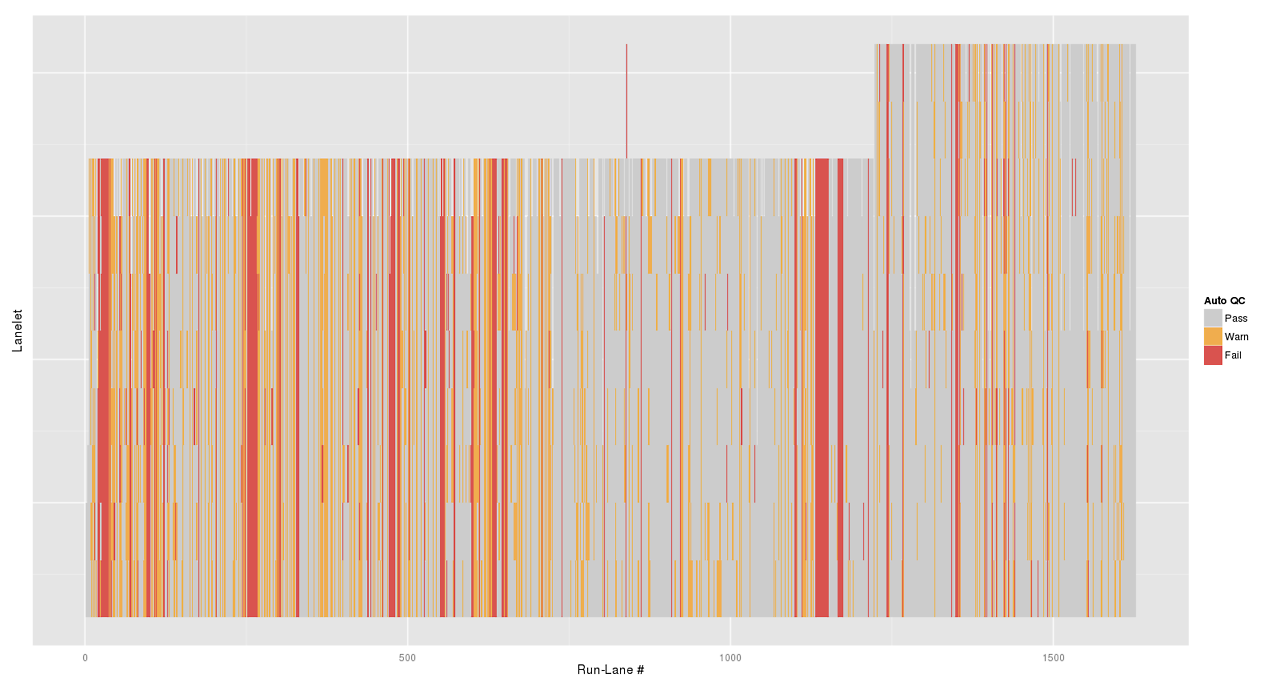
\includegraphics[width=1.0\textwidth]{classcorr}
    \caption[ClassCorr]{\textbf{Heatmap of lanelet QC status by lane}: Lanes are
    vertical bars with each lanelet cell coloured red to represent a failure,
yellow for a warning and grey for a pass.}
    \label{fig:classcorr}
\end{figure}

In such a case there would appear to exist a relationship between the respective
qualities of each lanelet in a lane as well as each lane in a sequencing run. To
examine this further, an R script utilising \textbf{ggplot2} was authored to
visually inspect whether correlation existed and if so to what degree that data
is affected.

Figure~\ref{fig:classcorr} displays a plot of \textbf{auto\_qc} classification
for each lanelet in a lane. The plot itself is a dense heatmap
where each lane stands as a vertical bar, broken into horizontal cells, each
of which represents a lanelet that was sequenced in that particular lane. These
lanelets are colour coded using; red for failures, yellow for warnings and grey
for passes (to allow the other two classes to be more easily seen).

Therefore an unbroken vertical red line indicates that all lanelets that
comprise of that line failed to pass some aspect of the current
\textbf{auto\_qc} thresholds. In reality there are few conditions under which
a lanelet would fail irrespective of the status of the rest of the lanelets in
the same lane which typically involve an error during the preparation of the
sample (an easy to spot result as it will cause poor quality across all lanelets
using that sample).

%TODO Better explanation
Overall there are a series of instances appearing to support correlation for
whole-lane failures and warnings but despite this there do appear to be occasions
where a lanelet has failed where the remainder of the lane has not.
Having discussed this with the project supervisor and contacts at the Sanger Institute we decided to continue to
the implementation stage, agreeing that whilst some evidence of correlation
between lanelets in the same lane has emerged, we will still be able to recover
parameters that will be useful to quality control and statistical testing may be
required following this analysis to describe how powerful such parameters are
taking this possible correlation into account.

It should be
noted that the proportion of failures and warnings is considerably smaller than
passes and so care will need to be taken to find a balance; for example it would
not be feasible to merely discard lanelets from lanes that have failed entirely
as there'd hardly be any data on which to train a classifier. Indeed other
solutions may be possible, perhaps weighting observations which exhibit similar
behaviour to other lanelets in their lane so as to give their parameter values
less priority during the construction of the classifier itself.

It is worth noting that although the plot does not make a particular
distinction between lanes in the same flow cell, lanes are sequentially
identified so the red bars of thicker-width arguably display some failures
across entire flow cells.

As a final note it should be stressed that this plot should be regarded as a
diagnostic rather than an experiment with a direct conclusion. Given more time it
would be useful to investigate the nature of these possible correlations, given
a lane that has failed across all lanelets: do those lanelets actually express
similar quality metrics?

%%%%%%%%%%%%%%%%%%%%%%%%%%%%%%%%%%%%%%%%%%%%%%%%%%%%%%%%%%%%%%%%%%%%%%%%%%%%%%%
\section{Recovering Ratios}
\label{app:ratios}

An initial scan of the summary numbers available in the "bamcheckr'd" files
introduced in Chapter~\ref{chap:bamcheckr-data} revealed 82 different
parameters. However, when comparing this parameter set to the threshold rules of
\textbf{auto\_qc}, it appeared that some parameters were "missing".

In the pursuit of replicating the decisions of the
existing system, it is ideal to have all the parameters used in the making of
those decisions at hand. In particular, the missing parameters were of a
normalised nature, typically in the form of a ratio or percentage which should
make them more valuable than a parameter that just represents a raw count of
some property.

It was found that these missing parameters are calculated in a step preceding
\textbf{auto\_qc} as part of the \textbf{vr-pipe}
pipeline\footnote{https://github.com/wtsi-hgi/vr-pipe/blob/hgi-release/modules/VRPipe/Steps/vrtrack\_auto\_qc\_hgi\_3.pm}.
Whilst I could have attempted to set-up my own instance of \textbf{vr-pipe} to
recover this data, speaking with contacts at the Sanger Institute, it was
decided that this would prove troublesome work; requiring an involved
deployment to a cloud based facility such as Amazon's Elastic Compute Cloud and
installation of various Perl dependencies as well as requiring access to many
controlled databases within the institute.

Most of the functions that calculated these parameters turned out to be
straightforward and could easily be ported to another application. At first
it was intended to add these functions to the program authored for this part of
the project, but the Sanger Institute suggested it would be more useful to
implement such functionality in \textbf{bamcheckr} directly, removing some of
\textbf{auto\_qc}'s dependence on its position in \textbf{vr-pipe}.

\begin{listing}[H]
    \caption[r-dev]{: Installing an in-development R package with \textbf{devtools}}
    \label{list:r-dev}
    \begin{minted}[mathescape,
                %linenos,
                numbersep=5pt,
                gobble=8,
                frame=lines,
                framesep=2mm]{r}
        # Install and include the `devtools' package
        install.packages("devtools")
        library(devtools)

        # Install package directly from Github repository
        install_github("samstudio8/seq_autoqc", subdir="bamcheckr")

        # Install package from local directory
        install("/home/sam/Projects/seq_autoqc/bamcheckr")

    \end{minted}
\end{listing}

With the help of \textbf{devtools}\citep{man:devtools} (see
Listing~\ref{list:r-dev}) it was simple to develop and test contributions to
\textbf{bamcheckr} locally without needing to re-publish the package after
changes. An additional script was added to \textbf{bamcheckr}'s NAMESPACE to
recover the missing ratio and percentage based parameters.

Unfortunately, the performance of the new script was poor, taking 5.5s on average
and increasing to 16.1s when enabling a complex function containing many vector
operations -- potentially inefficient due to my lack of R experience. It was
simply impractical to use \textbf{bamcheckr} to update thousands of files and
thus I instead used \textbf{Frontier} to load the "BAMcheckr'd" files and used
its API to calculate the missing parameters and write them back to the files.
An impressive feat for \textbf{Frontier} considering how simple it was to use it
for something it was not actually intended for.

An evaluation of the R language\citep{morandat-rperf} compares the language's
performance to both Python and C.
With such an intriguing difference in performance between \textbf{bamcheckr} and
\textbf{Frontier}, with significantly more
time it would be interesting to explore the idiosyncrasies of each
implementation.

